\begin{tikzpicture}
  \begin{scope}[on background layer]
      \node[anchor=south west,inner sep=0, opacity=0.8] at (0,0) {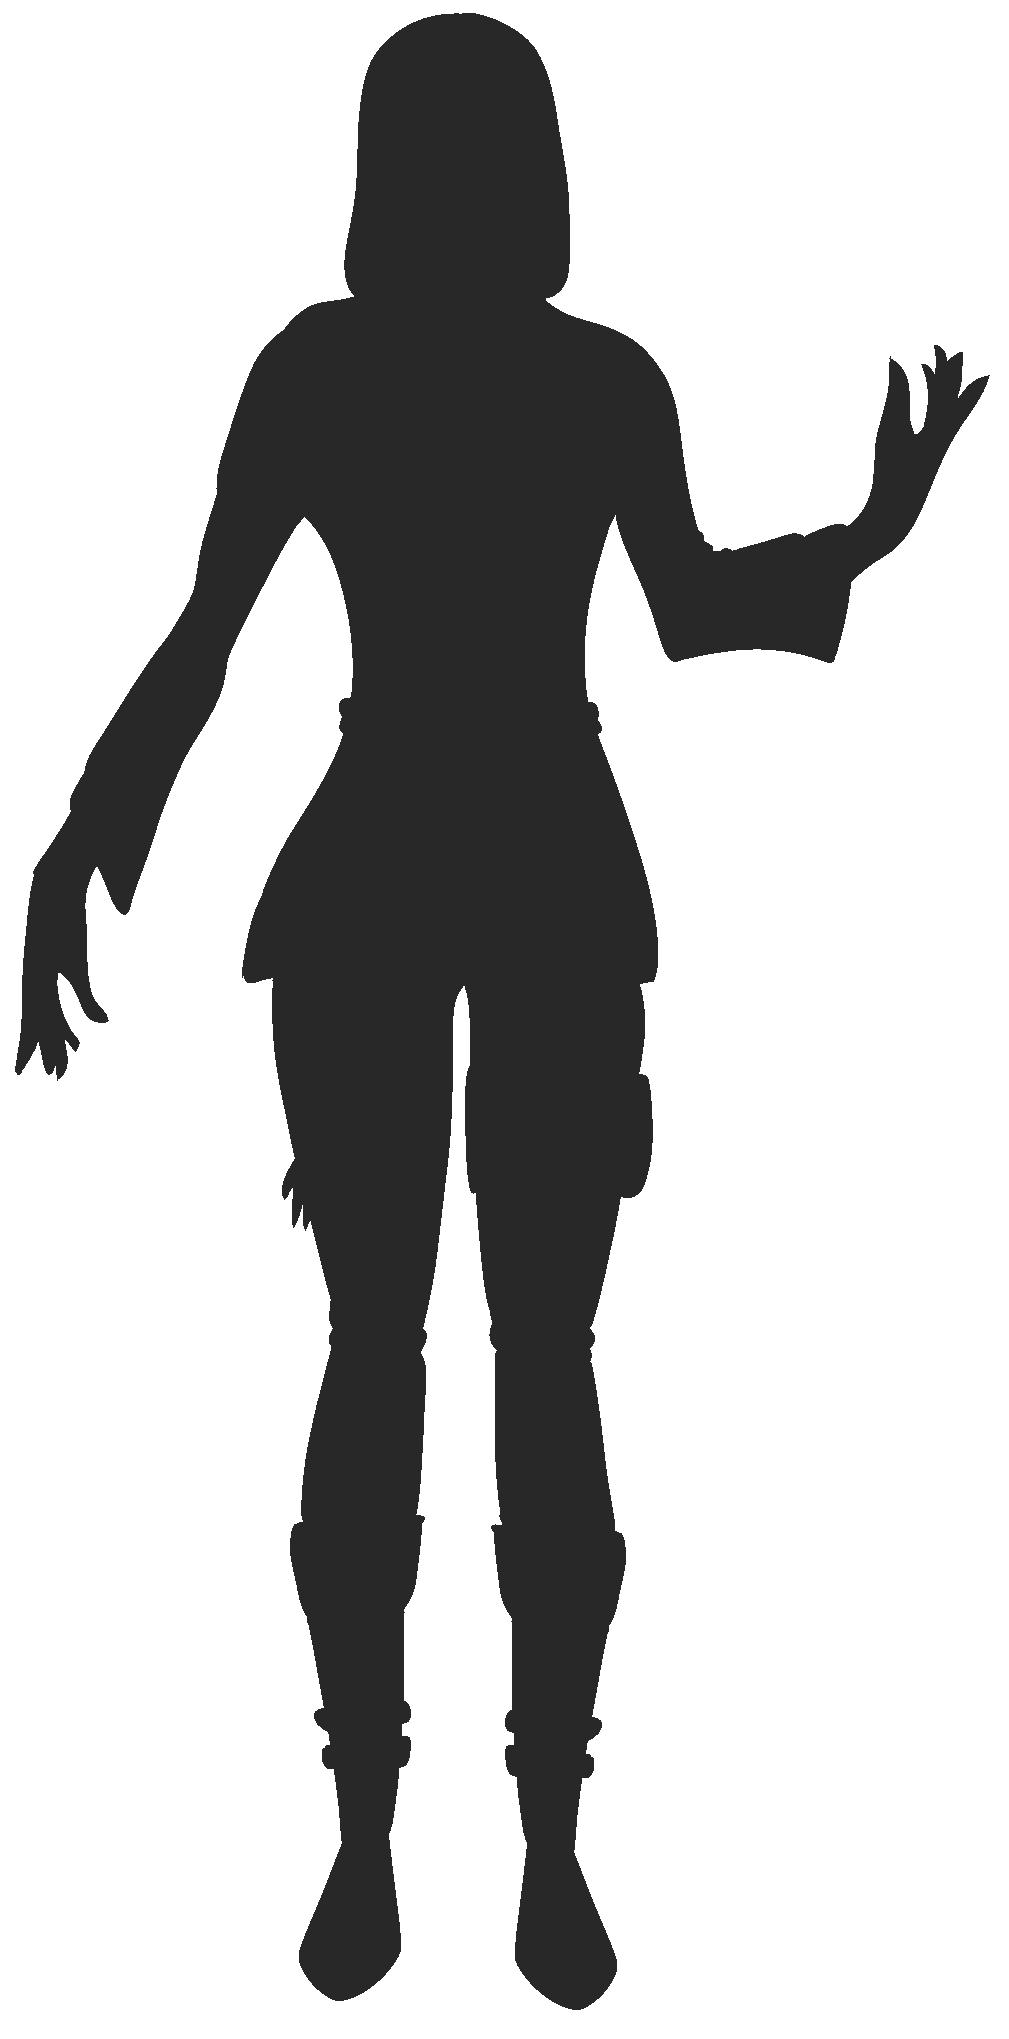
\includegraphics[width=6cm]{img/silhouette-w.png}};
  \end{scope}

  \node(kopf) at (2.75, 11) {\RS{Kopf}};
  \begin{scope}[on background layer]
      \path[fill=white, draw=black] ([yshift=0.1cm, xshift=0.2cm]kopf.north west) -- ([xshift=0.2cm]kopf.west) to[out=270, in=155] ([yshift=-0.1cm]kopf.south) to[out=25, in=270] ([xshift=-0.2cm]kopf.east) -- ([yshift=0.1cm, xshift=-0.2cm]kopf.north east) -- cycle;
  \end{scope}
  \node[below=2pt of kopf] {Ko};

  \filldraw[fill=white, draw=black] ([yshift=0.4cm]kopf.north) circle (0.2cm);
  \filldraw[fill=white, draw=black] ([yshift=0.4cm, xshift=0.5cm]kopf.north) circle (0.2cm);
  \filldraw[fill=white, draw=black] ([yshift=0.4cm, xshift=-0.5cm]kopf.north) circle (0.2cm);

  \node[minimum width=.4cm](brust) at (2.4, 9) {\RS{Brust}};
  \begin{scope}[on background layer]
      \path[fill=white, draw=black] ([yshift=0.1cm, xshift=0.2cm]brust.north west) -- ([xshift=0.2cm]brust.west) to[out=270, in=155] ([yshift=-0.1cm]brust.south) to[out=25, in=270] ([xshift=-0.2cm]brust.east) -- ([yshift=0.1cm, xshift=-0.2cm]brust.north east) -- cycle;
  \end{scope}
  \node[below=2pt of brust] {Br};
  \node[right=-4pt of brust](rucken) {\RS{Ruecken}};
  \begin{scope}[on background layer]
      \path[fill=white, draw=black] ([yshift=0.1cm, xshift=0.2cm]rucken.north west) -- ([xshift=0.2cm]rucken.west) to[out=270, in=155] ([yshift=-0.1cm]rucken.south) to[out=25, in=270] ([xshift=-0.2cm]rucken.east) -- ([yshift=0.1cm, xshift=-0.2cm]rucken.north east) -- cycle;
  \end{scope}
  \node[below=2pt of rucken] {Rü};

  \filldraw[fill=white, draw=black] ([yshift=0.4cm]$(brust.north)!0.5!(rucken.north)$) circle (0.2cm);
  \filldraw[fill=white, draw=black] ([yshift=0.4cm, xshift=0.5cm]$(brust.north)!0.5!(rucken.north)$) circle (0.2cm);
  \filldraw[fill=white, draw=black] ([yshift=0.4cm, xshift=-0.5cm]$(brust.north)!0.5!(rucken.north)$) circle (0.2cm);

  \node(larm) at (5.6, 8.5) {\RS{LArm}};
  \begin{scope}[on background layer]
      \path[fill=white, draw=black] ([yshift=0.1cm, xshift=0.2cm]larm.north west) -- ([xshift=0.2cm]larm.west) to[out=270, in=155] ([yshift=-0.1cm]larm.south) to[out=25, in=270] ([xshift=-0.2cm]larm.east) -- ([yshift=0.1cm, xshift=-0.2cm]larm.north east) -- cycle;
  \end{scope}
  \node[below=2pt of larm] {LA};

  \filldraw[fill=white, draw=black] ([yshift=-0.2cm, xshift=-0.2cm]larm.north west) circle (0.2cm);
  \filldraw[fill=white, draw=black] ([yshift=-0.2cm, xshift=-0.65cm]larm.north west) circle (0.2cm);
  \filldraw[fill=white, draw=black] ([yshift=-0.2cm, xshift=-1.1cm]larm.north west) circle (0.2cm);

  \node(rarm) at (0.8, 7) {\RS{RArm}};
  \begin{scope}[on background layer]
      \path[fill=white, draw=black] ([yshift=0.1cm, xshift=0.2cm]rarm.north west) -- ([xshift=0.2cm]rarm.west) to[out=270, in=155] ([yshift=-0.1cm]rarm.south) to[out=25, in=270] ([xshift=-0.2cm]rarm.east) -- ([yshift=0.1cm, xshift=-0.2cm]rarm.north east) -- cycle;
  \end{scope}
  \node[below=2pt of rarm] {RA};

  \filldraw[fill=white, draw=black] ([yshift=0.6cm, xshift=-0.3cm]rarm.north east) circle (0.2cm);
  \filldraw[fill=white, draw=black] ([yshift=1.1cm, xshift=-0.05cm]rarm.north east) circle (0.2cm);
  \filldraw[fill=white, draw=black] ([yshift=1.6cm, xshift=0.2cm]rarm.north east) circle (0.2cm);

  \node(bauch) at (2.75, 7.1) {\RS{Bauch}};
  \begin{scope}[on background layer]
      \path[fill=white, draw=black] ([yshift=0.1cm, xshift=0.2cm]bauch.north west) -- ([xshift=0.2cm]bauch.west) to[out=270, in=155] ([yshift=-0.1cm]bauch.south) to[out=25, in=270] ([xshift=-0.2cm]bauch.east) -- ([yshift=0.1cm, xshift=-0.2cm]bauch.north east) -- cycle;
  \end{scope}
  \node[below=2pt of bauch] {Ba};

  \filldraw[fill=white, draw=black] ([yshift=0.4cm]bauch.north) circle (0.2cm);
  \filldraw[fill=white, draw=black] ([yshift=0.4cm, xshift=0.5cm]bauch.north) circle (0.2cm);
  \filldraw[fill=white, draw=black] ([yshift=0.4cm, xshift=-0.5cm]bauch.north) circle (0.2cm);

  \node(rbein) at (2.1, 3) {\RS{RBein}};
  \begin{scope}[on background layer]
      \path[fill=white, draw=black] ([yshift=0.1cm, xshift=0.2cm]rbein.north west) -- ([xshift=0.2cm]rbein.west) to[out=270, in=155] ([yshift=-0.1cm]rbein.south) to[out=25, in=270] ([xshift=-0.2cm]rbein.east) -- ([yshift=0.1cm, xshift=-0.2cm]rbein.north east) -- cycle;
  \end{scope}
  \node[below=2pt of rbein] {RB};

  \filldraw[fill=white, draw=black] ([yshift=0.8cm, xshift=0.12cm]rbein.north) circle (0.2cm);
  \filldraw[fill=white, draw=black] ([yshift=1.5cm, xshift=0.18cm]rbein.north) circle (0.2cm);
  \filldraw[fill=white, draw=black] ([yshift=2.2cm, xshift=0.24cm]rbein.north) circle (0.2cm);

  \node(lbein) at (3.3, 3) {\RS{LBein}};
  \begin{scope}[on background layer]
      \path[fill=white, draw=black] ([yshift=0.1cm, xshift=0.2cm]lbein.north west) -- ([xshift=0.2cm]lbein.west) to[out=270, in=155] ([yshift=-0.1cm]lbein.south) to[out=25, in=270] ([xshift=-0.2cm]lbein.east) -- ([yshift=0.1cm, xshift=-0.2cm]lbein.north east) -- cycle;
  \end{scope}
  \node[below=2pt of lbein] {LB};

  \filldraw[fill=white, draw=black] ([yshift=0.8cm, xshift=-0cm]lbein.north) circle (0.2cm);
  \filldraw[fill=white, draw=black] ([yshift=1.5cm, xshift=-0cm]lbein.north) circle (0.2cm);
  \filldraw[fill=white, draw=black] ([yshift=2.2cm, xshift=-0cm]lbein.north) circle (0.2cm);
\end{tikzpicture}